\chapter{Infectome pipeline}

\section{Cell-free DNA}

In 1947, Mandel and Metais first observed that human blood contains circulating cell-free DNA molecules. These fragments enter blood as the detritus of dead cells and circulate with short (15 minute) half-life as nucleosome-protected fragments \cite{Quake:2012iy}. Methods of molecular counting (notably NGS) have taken advantage of this phenomenon, as the abundance of cell-free DNA species may correlate with human health. Their greatest value has been to measure the proportion of foreign genomes within an individual. Cancer-associated mutations can be used to determine the progress of disease \cite{Newman:2014ik}, fetal DNA assayed by molecular counting can be used to detect aneuploidies (such as Down syndrome) \cite{Fan:2008ww}, and donor-organ derived DNA fragments can be monitored as marker of rejection following transplantation \cite{DeVlaminck:2013hl}. One critical advantage in all cases is that these measurements are non-invasive. 

The ability to resolve foreign genomes in blood presents an opportunity for infectious disease monitoring. The broad case for NGS in infectious disease diagnostics is already clear, particularly considering the growing importance of human microbiome on human health \cite{Consortium:2012bb}. The application of NGS to micro-organism derived cell-free DNA fragments presents two new opportunities for infection monitoring: (1) Translocation of micro-organisms from body sites, such as the GI tract, into the systemic circulation is known to occur and often has detrimental consequences, including immune activation or, in extreme cases, septic shock \cite{Brenchley:2012bm}. Direct measurement of composition in blood may be used to monitor active microbial translocation due to pathological damange of organ integrity. (2) Cell death and percolation of microbial products into blood may indicate the presence of infections compartmentalized within body sites, including deep tissues that are otherwise hard to access.

Recent work has shown that micro-organism derived cell-free DNA fragments do indeed exist and can be counted using NGS \cite{DeVlaminck:2013hl}. In turn, a critical question is whether these micro-organism derived cell-free DNA fragments are indicative of pathology within specific organ systems. In principle, these measurements can correlated with independent clinical tests of infetion establish their clinical relevance.

\section{Pipeline for the cell-free microbiome}

Prior to establishing the clinical relevance of micro-organism derived cell-free DNA, we built a computational pipeline and application for processing and analyzing the data, respectively. The general strategy for cell-free DNA isolation, sequencing, and read assignment have all been well-described \cite{DeVlaminck:2013hl}. First, human-derived reads are subtracted computationally using a short-read alignment algorithm (e.g, Bowtie). This step is followed by alignment (e.g., BLAST) to a reference database that contains sequences from candidate pathogens (e.g., NCBI). Algorithms to reduce ambiguity in these alignments \cite{Xia:2011it} may also be employed. In spite of this, four challenges must be acknowledged in pipeline and application design.

\textbf{Large data}: Alignment algorithms must contend with large amounts of sequence data. For example, the Illumina Next-Seq can now output >100 gigabases (Gb) of reads per day. Furthermore, reference databases of host and pathogen sequences used by BLAST range in size from 2 Gb for viruses to 3.1 Gb for the human genome and 42 Gb for all nucleotide sequences in the National Center for Biotechnology Information (NCBI) nucleotide (nt) collection (as of January 2013). 

\begin{figure*}
\center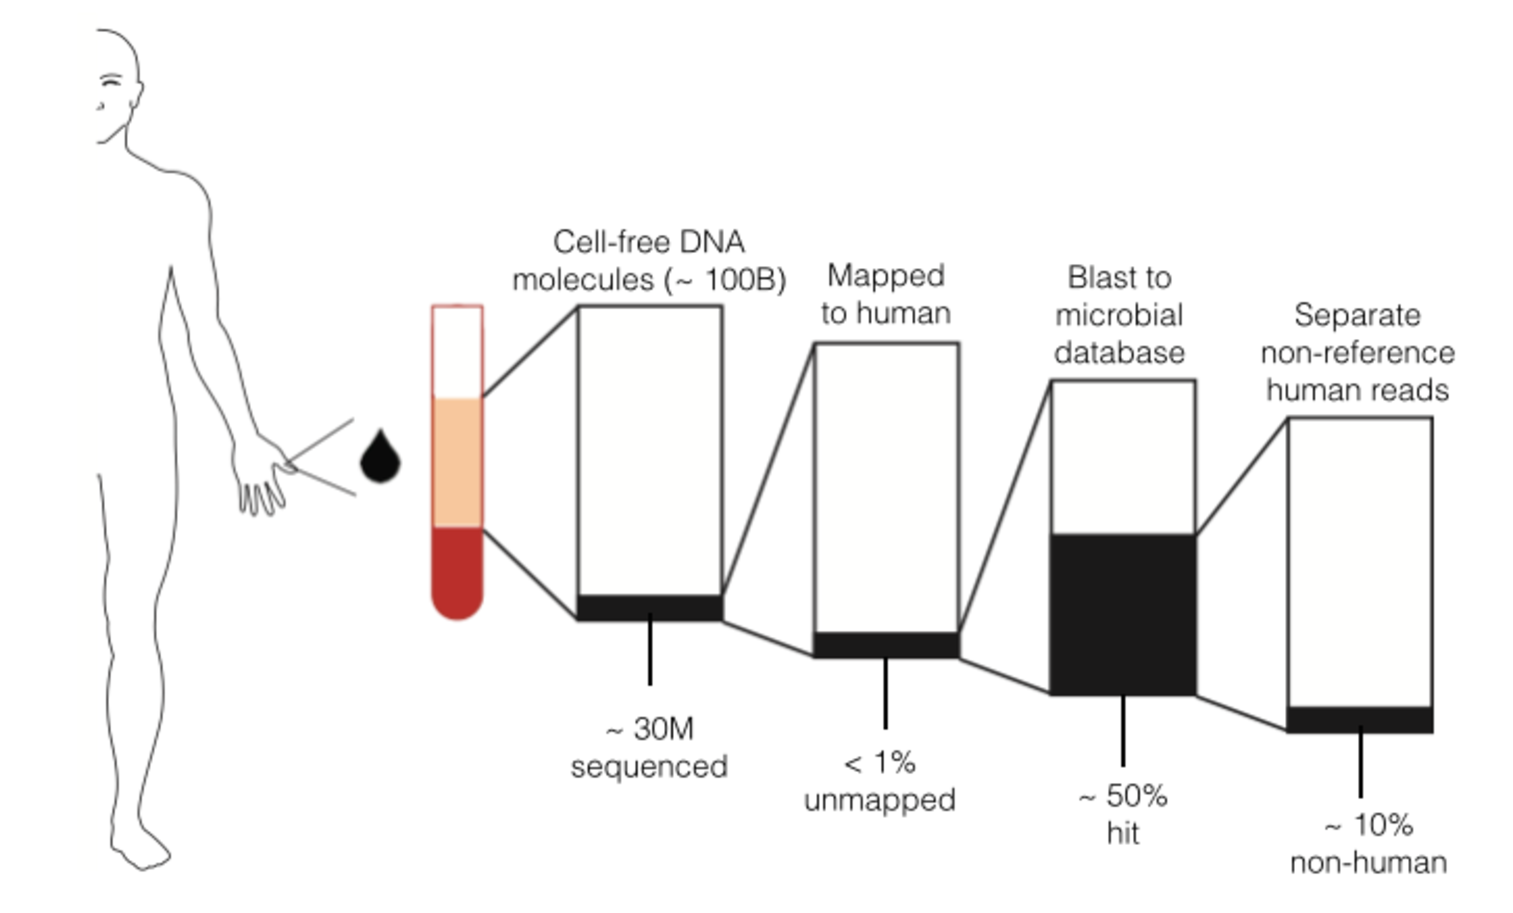
\includegraphics[width=120mm,scale=0.5]{Figures/Fig3}
\caption{Isolation of non-human cell-free DNA.}
\label{fig:Fig3}
\end{figure*}

\textbf{Signal}: In general, only a small fraction of NGS reads in clinical meta-genomic data correspond to pathogens \cite{Naccache:2014gk}. This is particularly true in the case of cell-free DNA, as non-human cell-free DNA is typically < 1\% of reads based upon initial human subtraction (e.g., mapping to the human genome). Furthermore, only a fraction of the un-mapped reads are derived from non-human sources, as most are either human-derived fragments that are not found in the human reference or do not align to the BLAST database used after mapping (Figure ~\ref{fig:Fig3}). 

\textbf{Speed}: BLAST is likely too slow for routine clinical analysis of NGS metagenomics data, as end-to-end processing times, even on multicore computational servers, can take several days to weeks.  Analysis pipelines that use faster, albeit less sensitive, algorithms upfront for host computational subtraction, such as PathSeq, still rely on traditional BLAST approaches for final pathogen determination.  

\textbf{Interpretation}: the data must bed organized and presented at scale, across large clinical cohorts, such that it is intuitive for researchers and clinicians.

The signal problem will be addressed through bio-chemical methods to enrich for non-human derived nucleic acids. Furthermore, the speed problem has recently been addressed using faster alignment algorithms, such as SNAP in place of BLAST and RAPSearch for assignment of de novo contig assemblies in order to classify potentially novel organisms \cite{Naccache:2014gk}. Despite these technical advances, there will probably continue to be a gap between the availability of such data and the ability to comprehensively interpret the results for clinical decision making. 

With this in mind, our emphasis was to develop a full application stack that performed both processing as well as data organization and visualization to aid with interpretation of the results. In order to achieve this, we built a pipeline comprised of cluster scripts that execute alignment, BLAST, and associated clean-up scripts \cite{Xia:2011it}. We then build an application stack on top of this pipeline written in Python, using a Postgres relational database as the store for relevant pipeline-specific reference files (e.g., taxonomic table), outputs (e.g., BLAST results), and sample -meta data. We wrote the application using the Django web-development framework with the Matplotlib visualization library \cite{Hunter:2007ux} and the Pandas library for data analysis, and Sqlalchemy for integration with Postgres (Figure ~\ref{fig:Fig4}).

\begin{figure*}
\center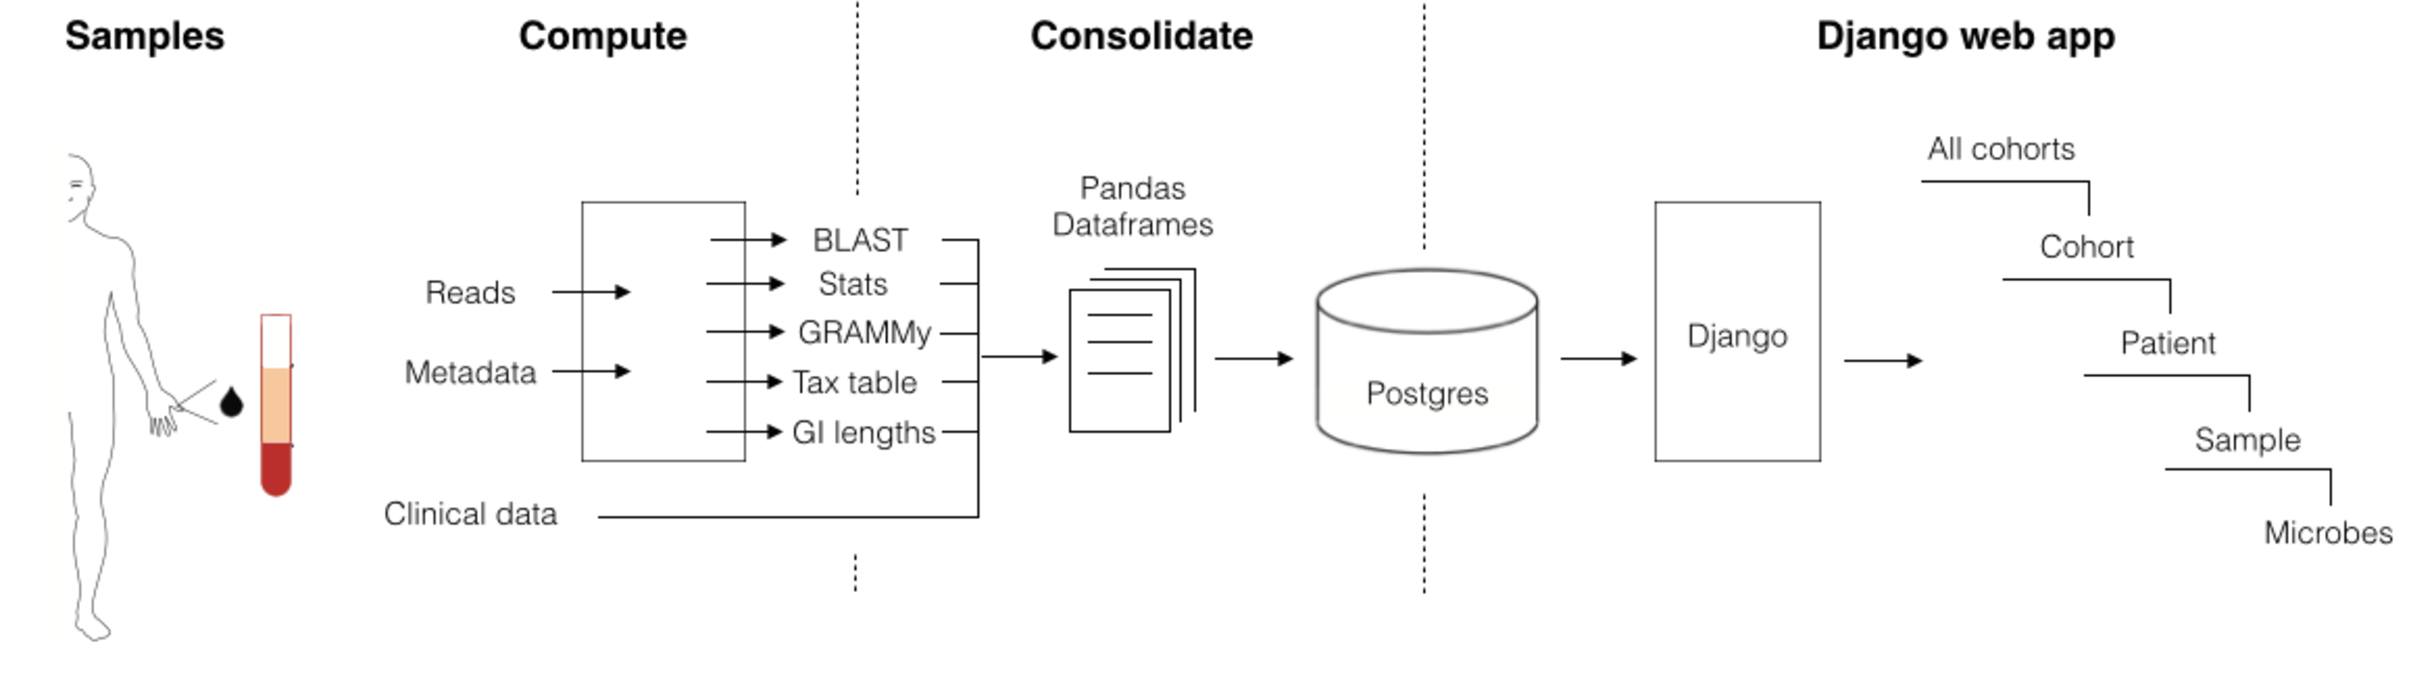
\includegraphics[width=150mm,scale=0.5]{Figures/Fig4}
\caption{Django application for infectome data.}
\label{fig:Fig4}
\end{figure*}

We processed several thousands cell-free DNA samples for different clinical cohorts using this pipeline. Each cohort was comprised of patients, which in turn may have many samples. In each sample, there may be thousands of unique infections identified in the cell-free DNA sequencing. Furthermore, infections may be viewed at different levels of taxonomic complexity, such as genus or species level resolution. 

With this in mind, we designed our application for intuitive navigation of this multi-scale data and were influenced by a rich history of genomic data browsers, which have been useful tools for navigating genomic data since the early 2000s \cite{ODonoghue:2010bd}. The Django application presents a series of web pages that reflect each level of organization in the data for intuitive browsing by researchers and clinicians.

The cohort page is the top level of organization in the application. It presents a table of patients, which is sorted by the number of samples per patient and provides a link to explore data for each patient in the cohort. It also provides cohort-level histograms that explain the incidence of each infection in the cohort (fraction of samples in which an infection is found) as well as the load per sample (the number of infections identified per sample). In addition, the cohort page provides a table of infections sorted by prevalence within the cohort. Finally, it provides a toggle that allows the data to be presented at different levels of taxonomic resolution, from genus to species (Figure ~\ref{fig:Fig5}). This make it possible to navigate the data in two ways: it is possible to take a patient-centric approach and examine specified patients (via the patient table) or an infection-centric approach (via infection table).

\begin{figure*}
\center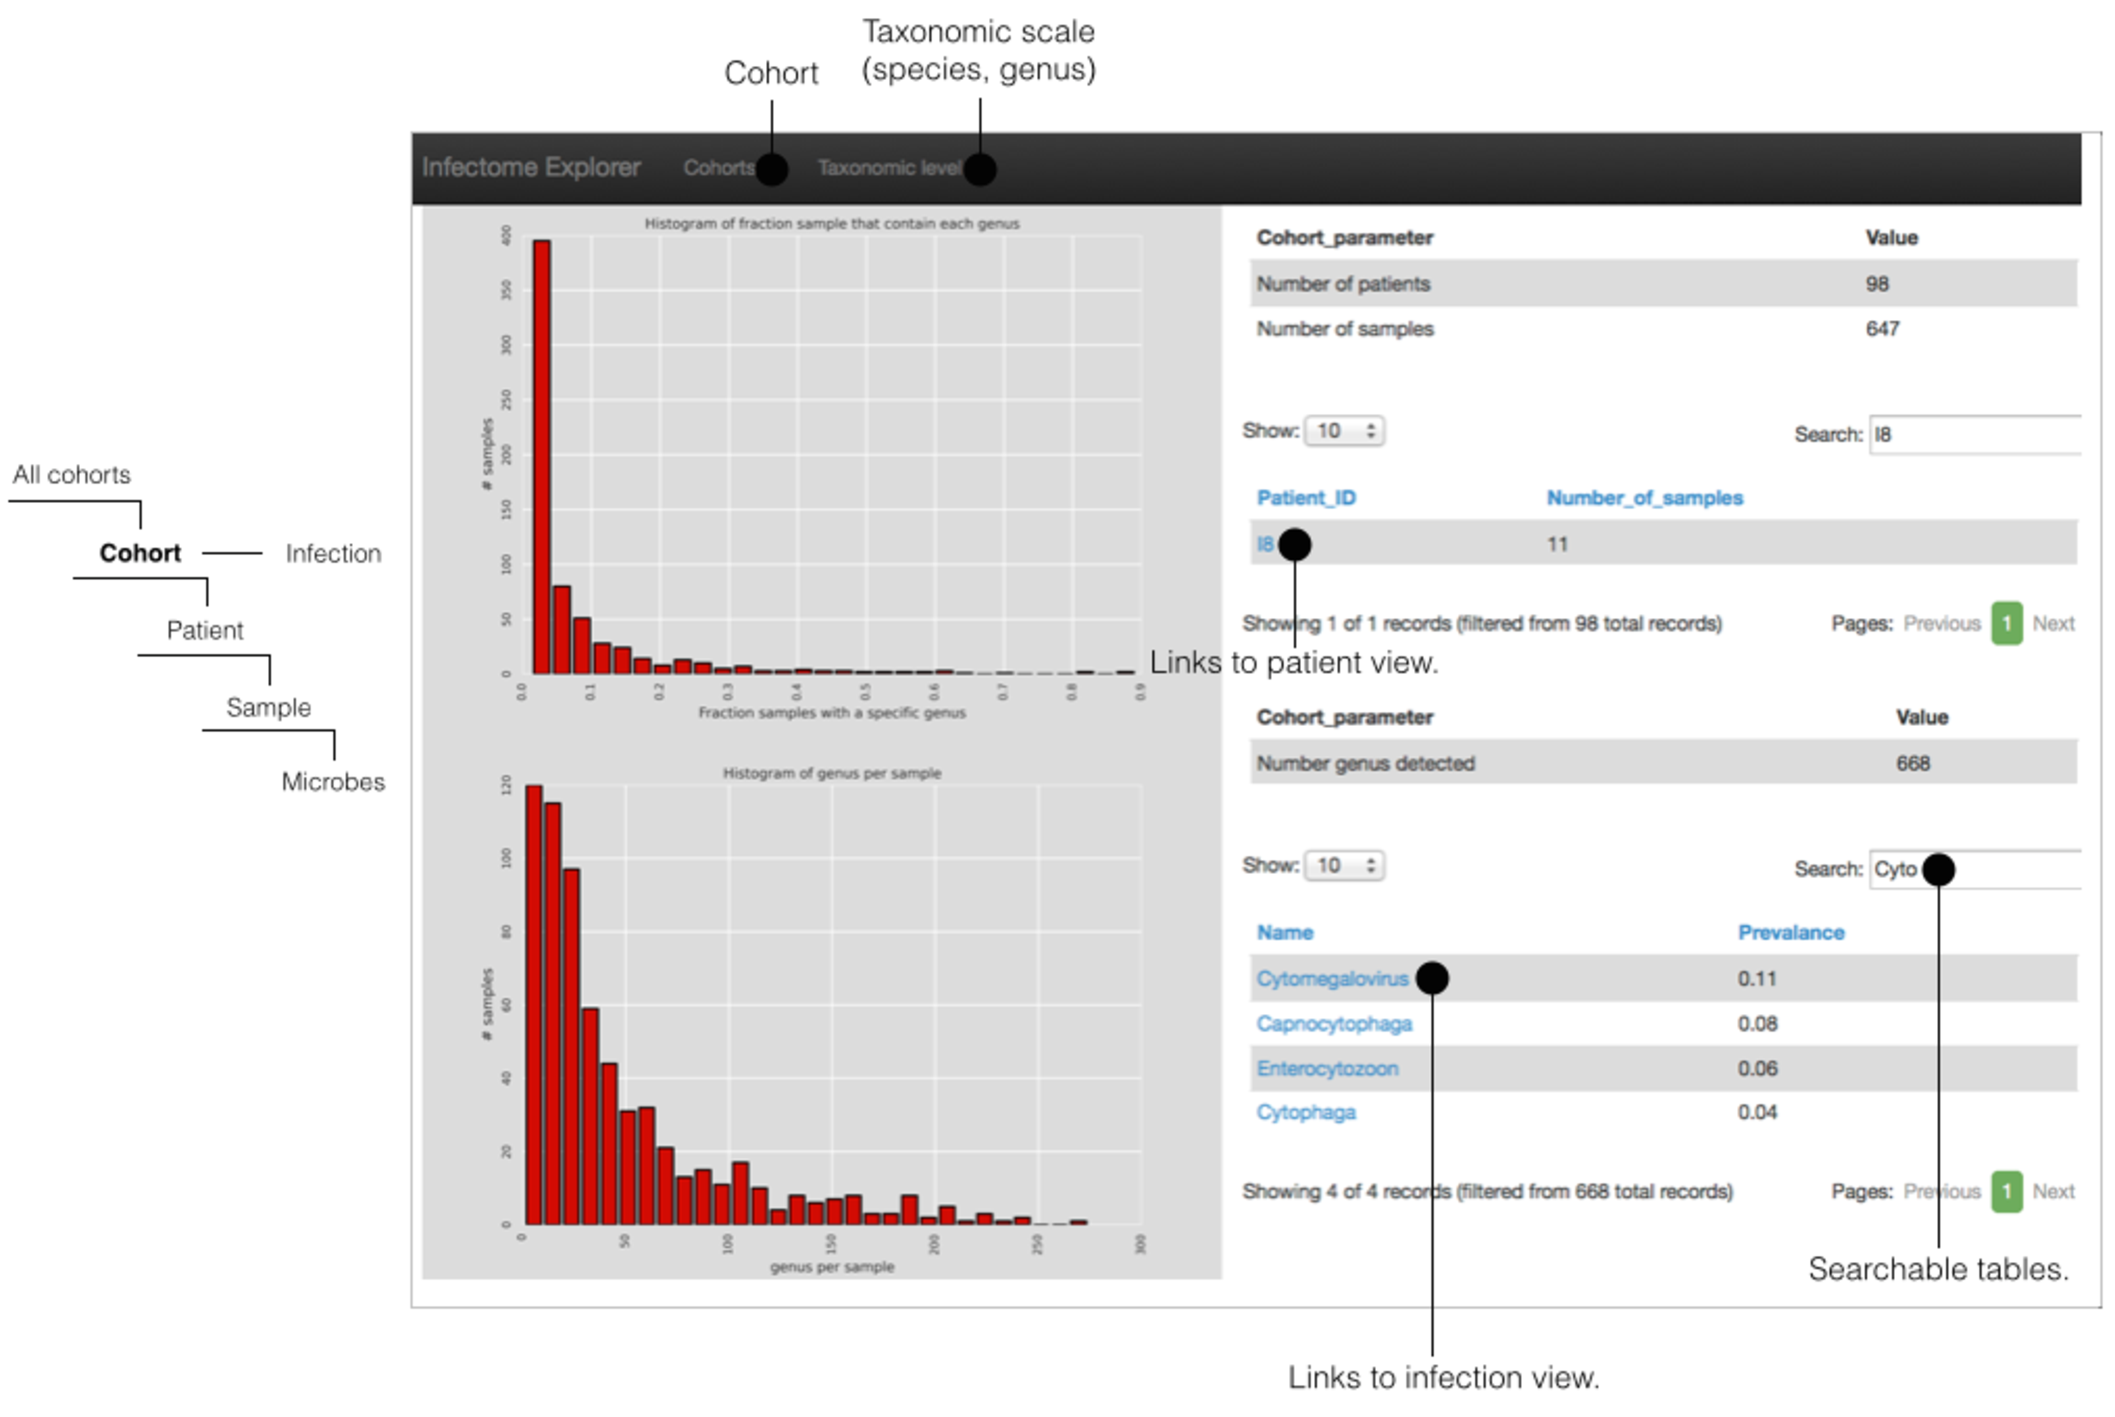
\includegraphics[width=150mm,scale=0.5]{Figures/Fig5}
\caption{Cohort view in the infectome application.}
\label{fig:Fig5}
\end{figure*}

The patient-centric approach can be used to quickly identify the infections identified within a specified patient at a specified taxonomic scale (e.g., genus or species). In order to present this information intuitively, we transform the raw abundance measurements returned by the sequencing pipeline The pipeline uses an algorithm (GRAMMy) to process the raw BLAST results; GRAMMy addresses two problems. 

First, each organism has a different genome size and, in turn, genome size affects the number of reads expected for each. Second, reads often align to multiple genomes. Taking these into account, GRAMMy performs a maximum likelihood estimation for read assignment to each organism and provides relative abundance measurement per organism within each cell-free DNA sample. 

From this measurment, we compute an estimate for absolute read counts per each identified genome. With this value, we then compute a coverage ratio between the infection and the human for that sample. We scale this value by $10^6$, resulting in relative genome copies per million ($gcm$). In isolation, this value is reasonably intuitive: it indicates the number of genome copies for a given infection relative to sampled human-derived reads in that sample. A ratio of $1$, for example, means that sampled organism genome copies is equivalent to sampled human genome copies. 

For presentation, the raw $gcm$ value may not be informative: a large value may be use we convert this value into a percentile (Figure ~\ref{fig:Fig6}) with respect to the full cohort for that particular infection. The percentile value simply indicates the magnitude of each measurement relative to what was observed across the cohort. 

\begin{figure*}
\center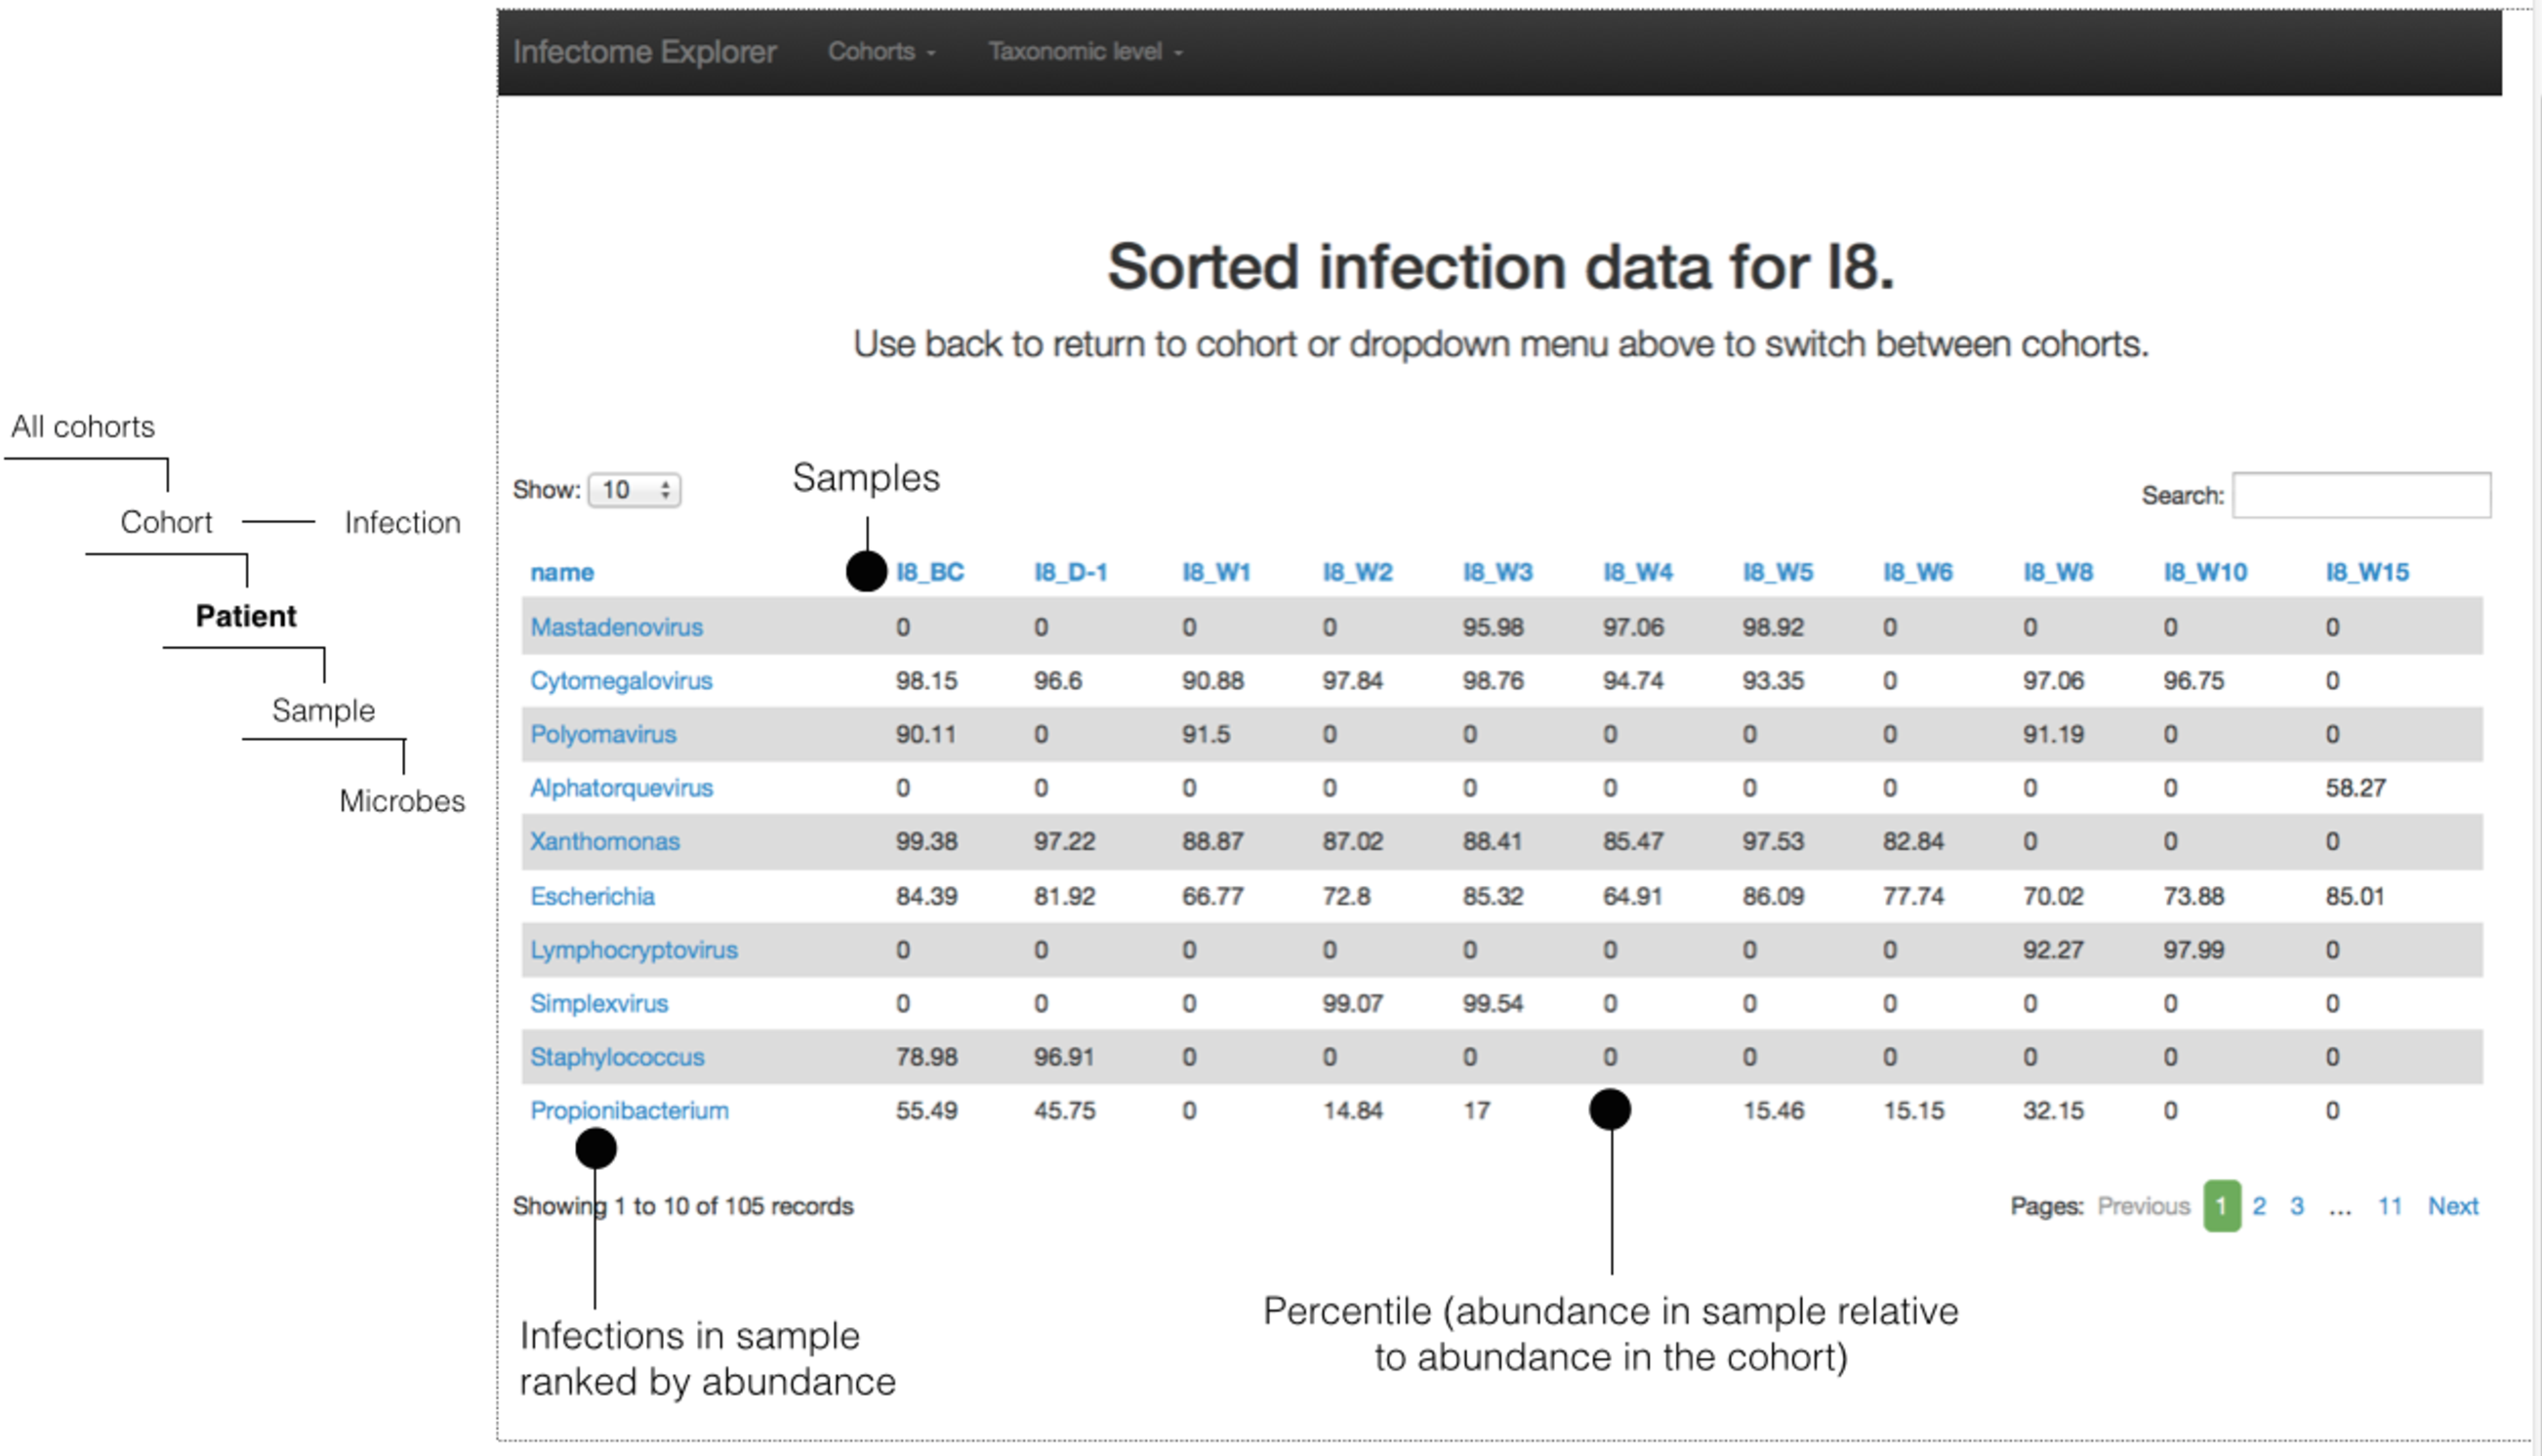
\includegraphics[width=150mm,scale=0.5]{Figures/Fig6}
\caption{Patient view in the infectome application.}
\label{fig:Fig6}
\end{figure*}

From the patient view, it is possible to drill down into each identified infection. In this case, it is useful to know both time-series data for that infection as well as detailed information about read coverage across the microbial genome. Both measurements can provide greater confidence about a given signal. For example, a consistent infection timeseries across samples supports likelihood of a bona-fire infection relative to a spurious signal found in one sample.

Furthermore, coverage is computed directly from the raw BLAST data. The BLAST file provides an alignment of each read to a particular GIs (individual sequence record in the BLAST database). GIs are associated with NCBI taxIDs, which are unique identifiers for micro-organisms. We aggregate GIs present in the BLAST file by taxID. We concatenate GIs into a composite track for the associated taxID.

\begin{figure*}
\center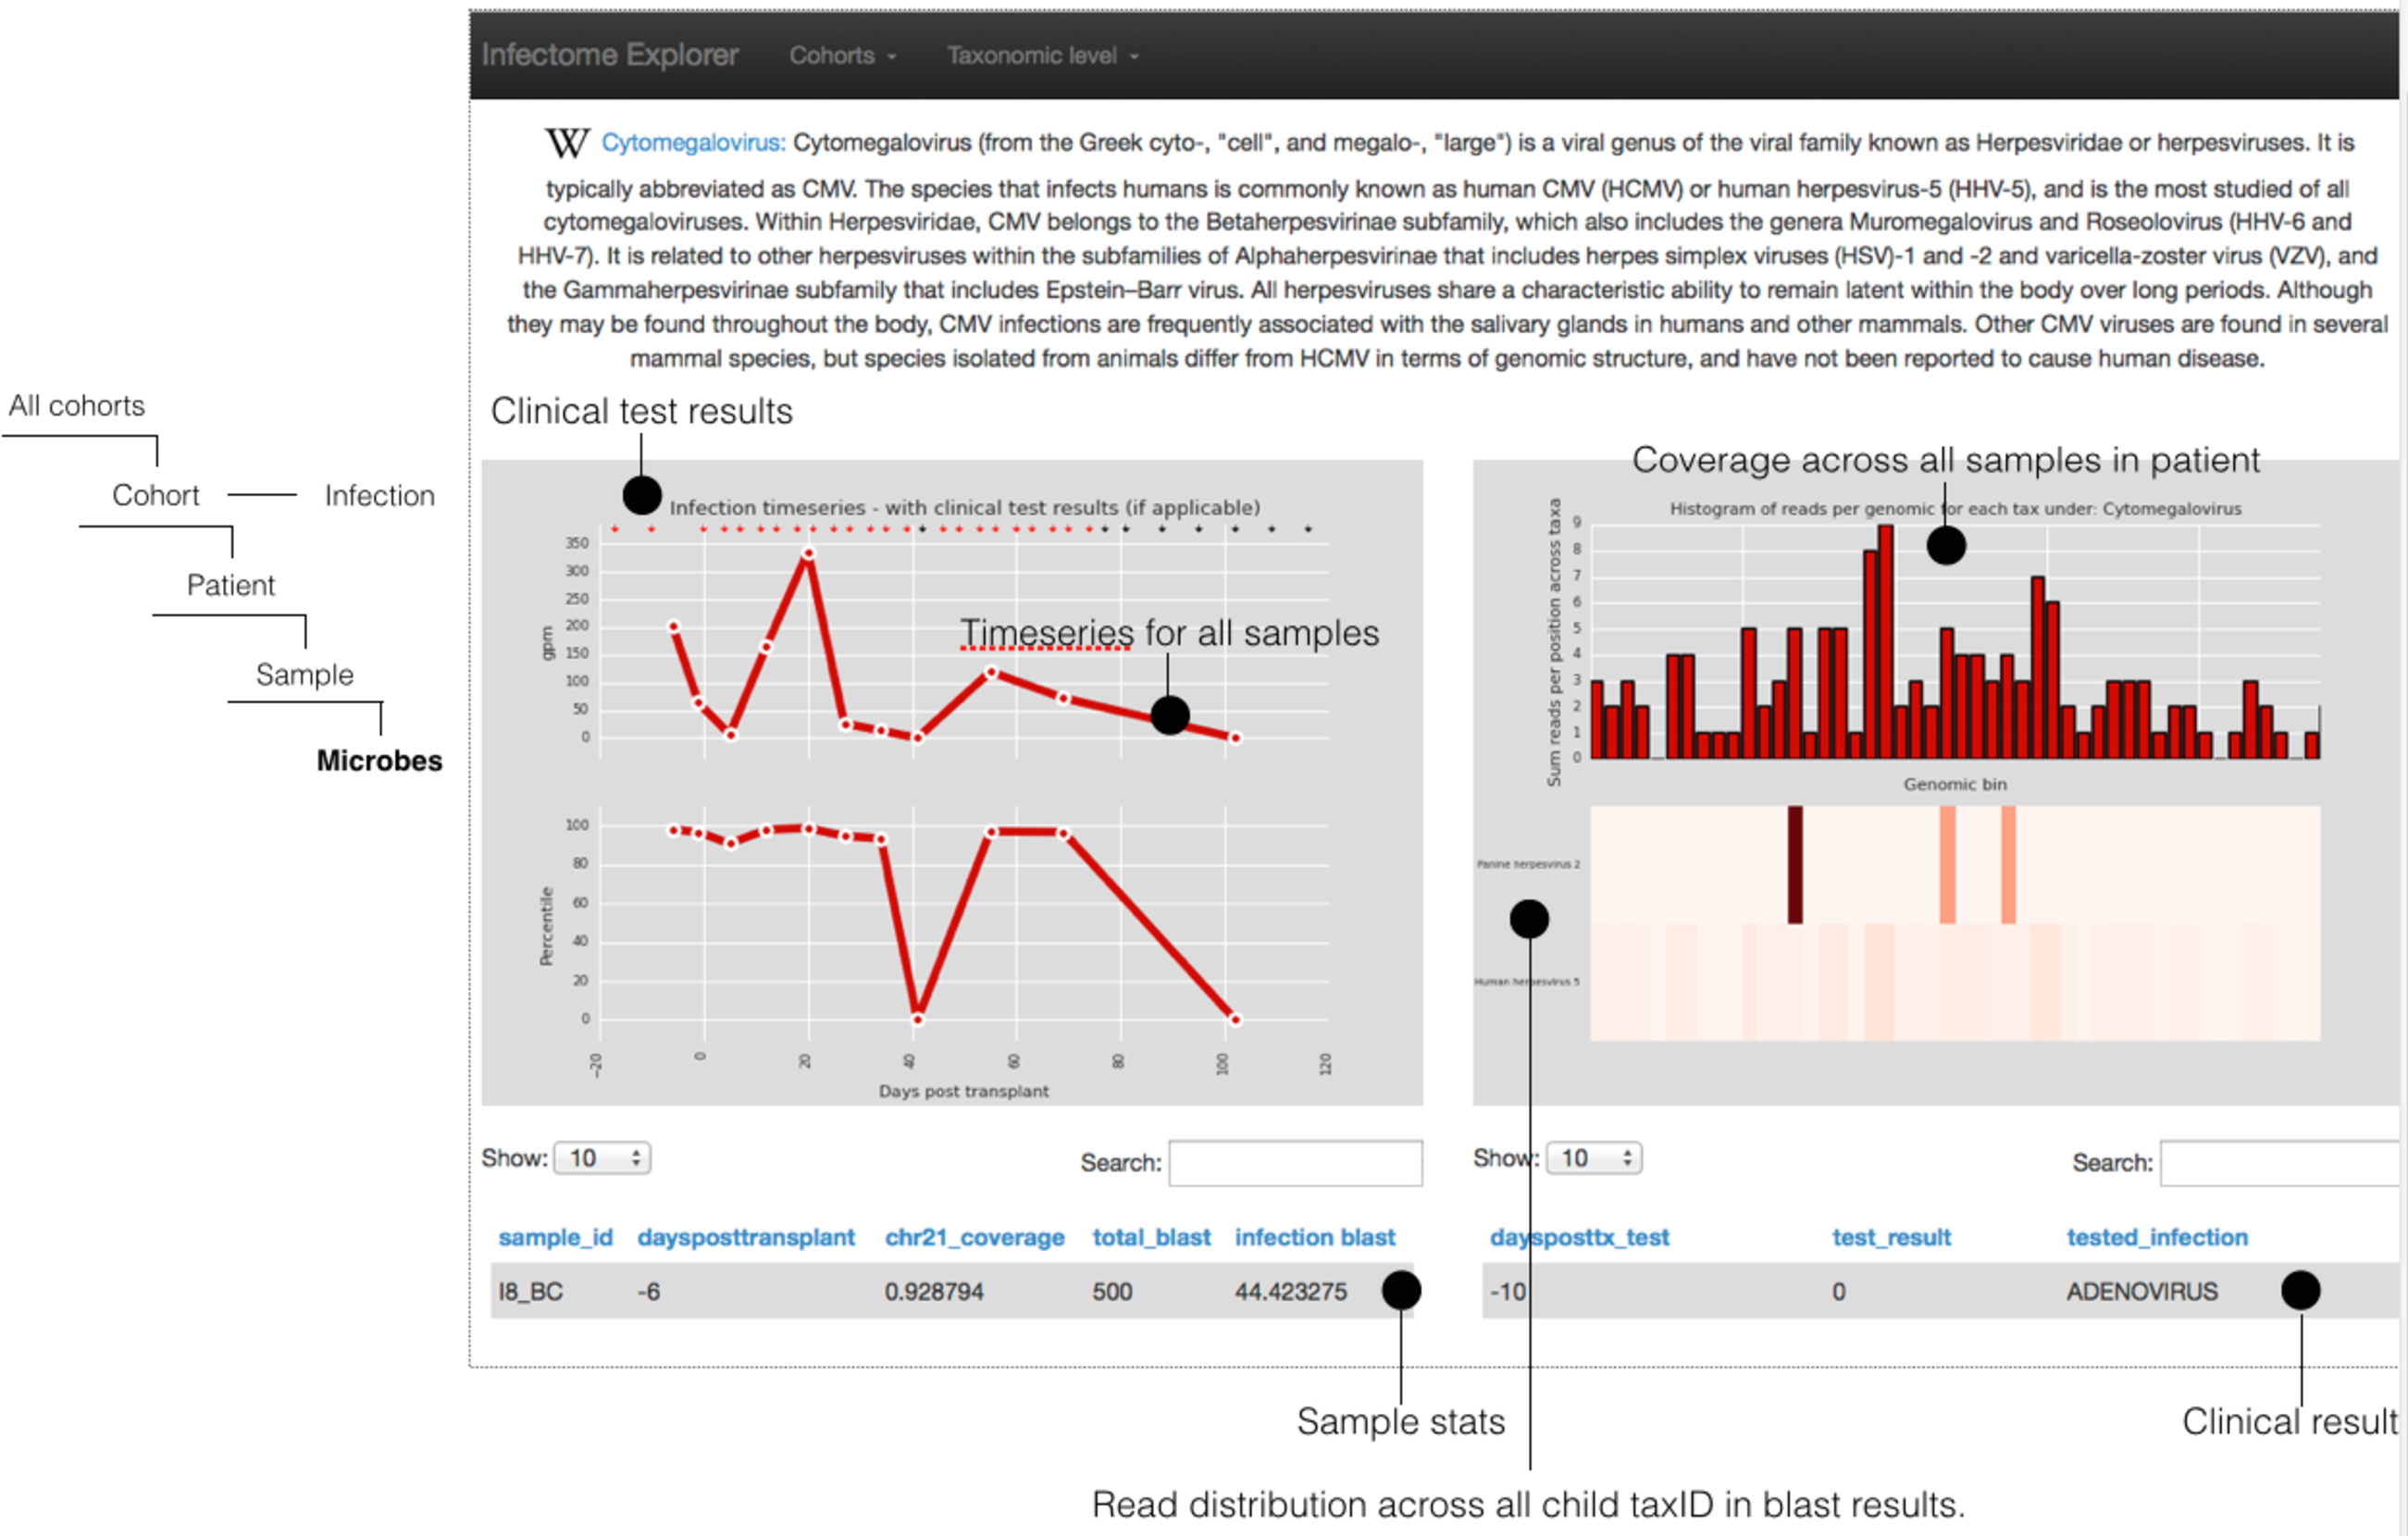
\includegraphics[width=150mm,scale=0.5]{Figures/Fig7}
\caption{Infection view in the infectome application.}
\label{fig:Fig7}
\end{figure*}

We then compute the mapping position of all reads within the composite genome. Irregular coverage patters may be indicative of database contamination, as this may mean that all reads align only to a single GI associated with a given infection or may align to a narrow region within a given GI. Using data from a bone marrow transplant cohort patient (I8), we show both timeseries and coverage data (Figure ~\ref{fig:Fig7}).

\begin{figure*}
\center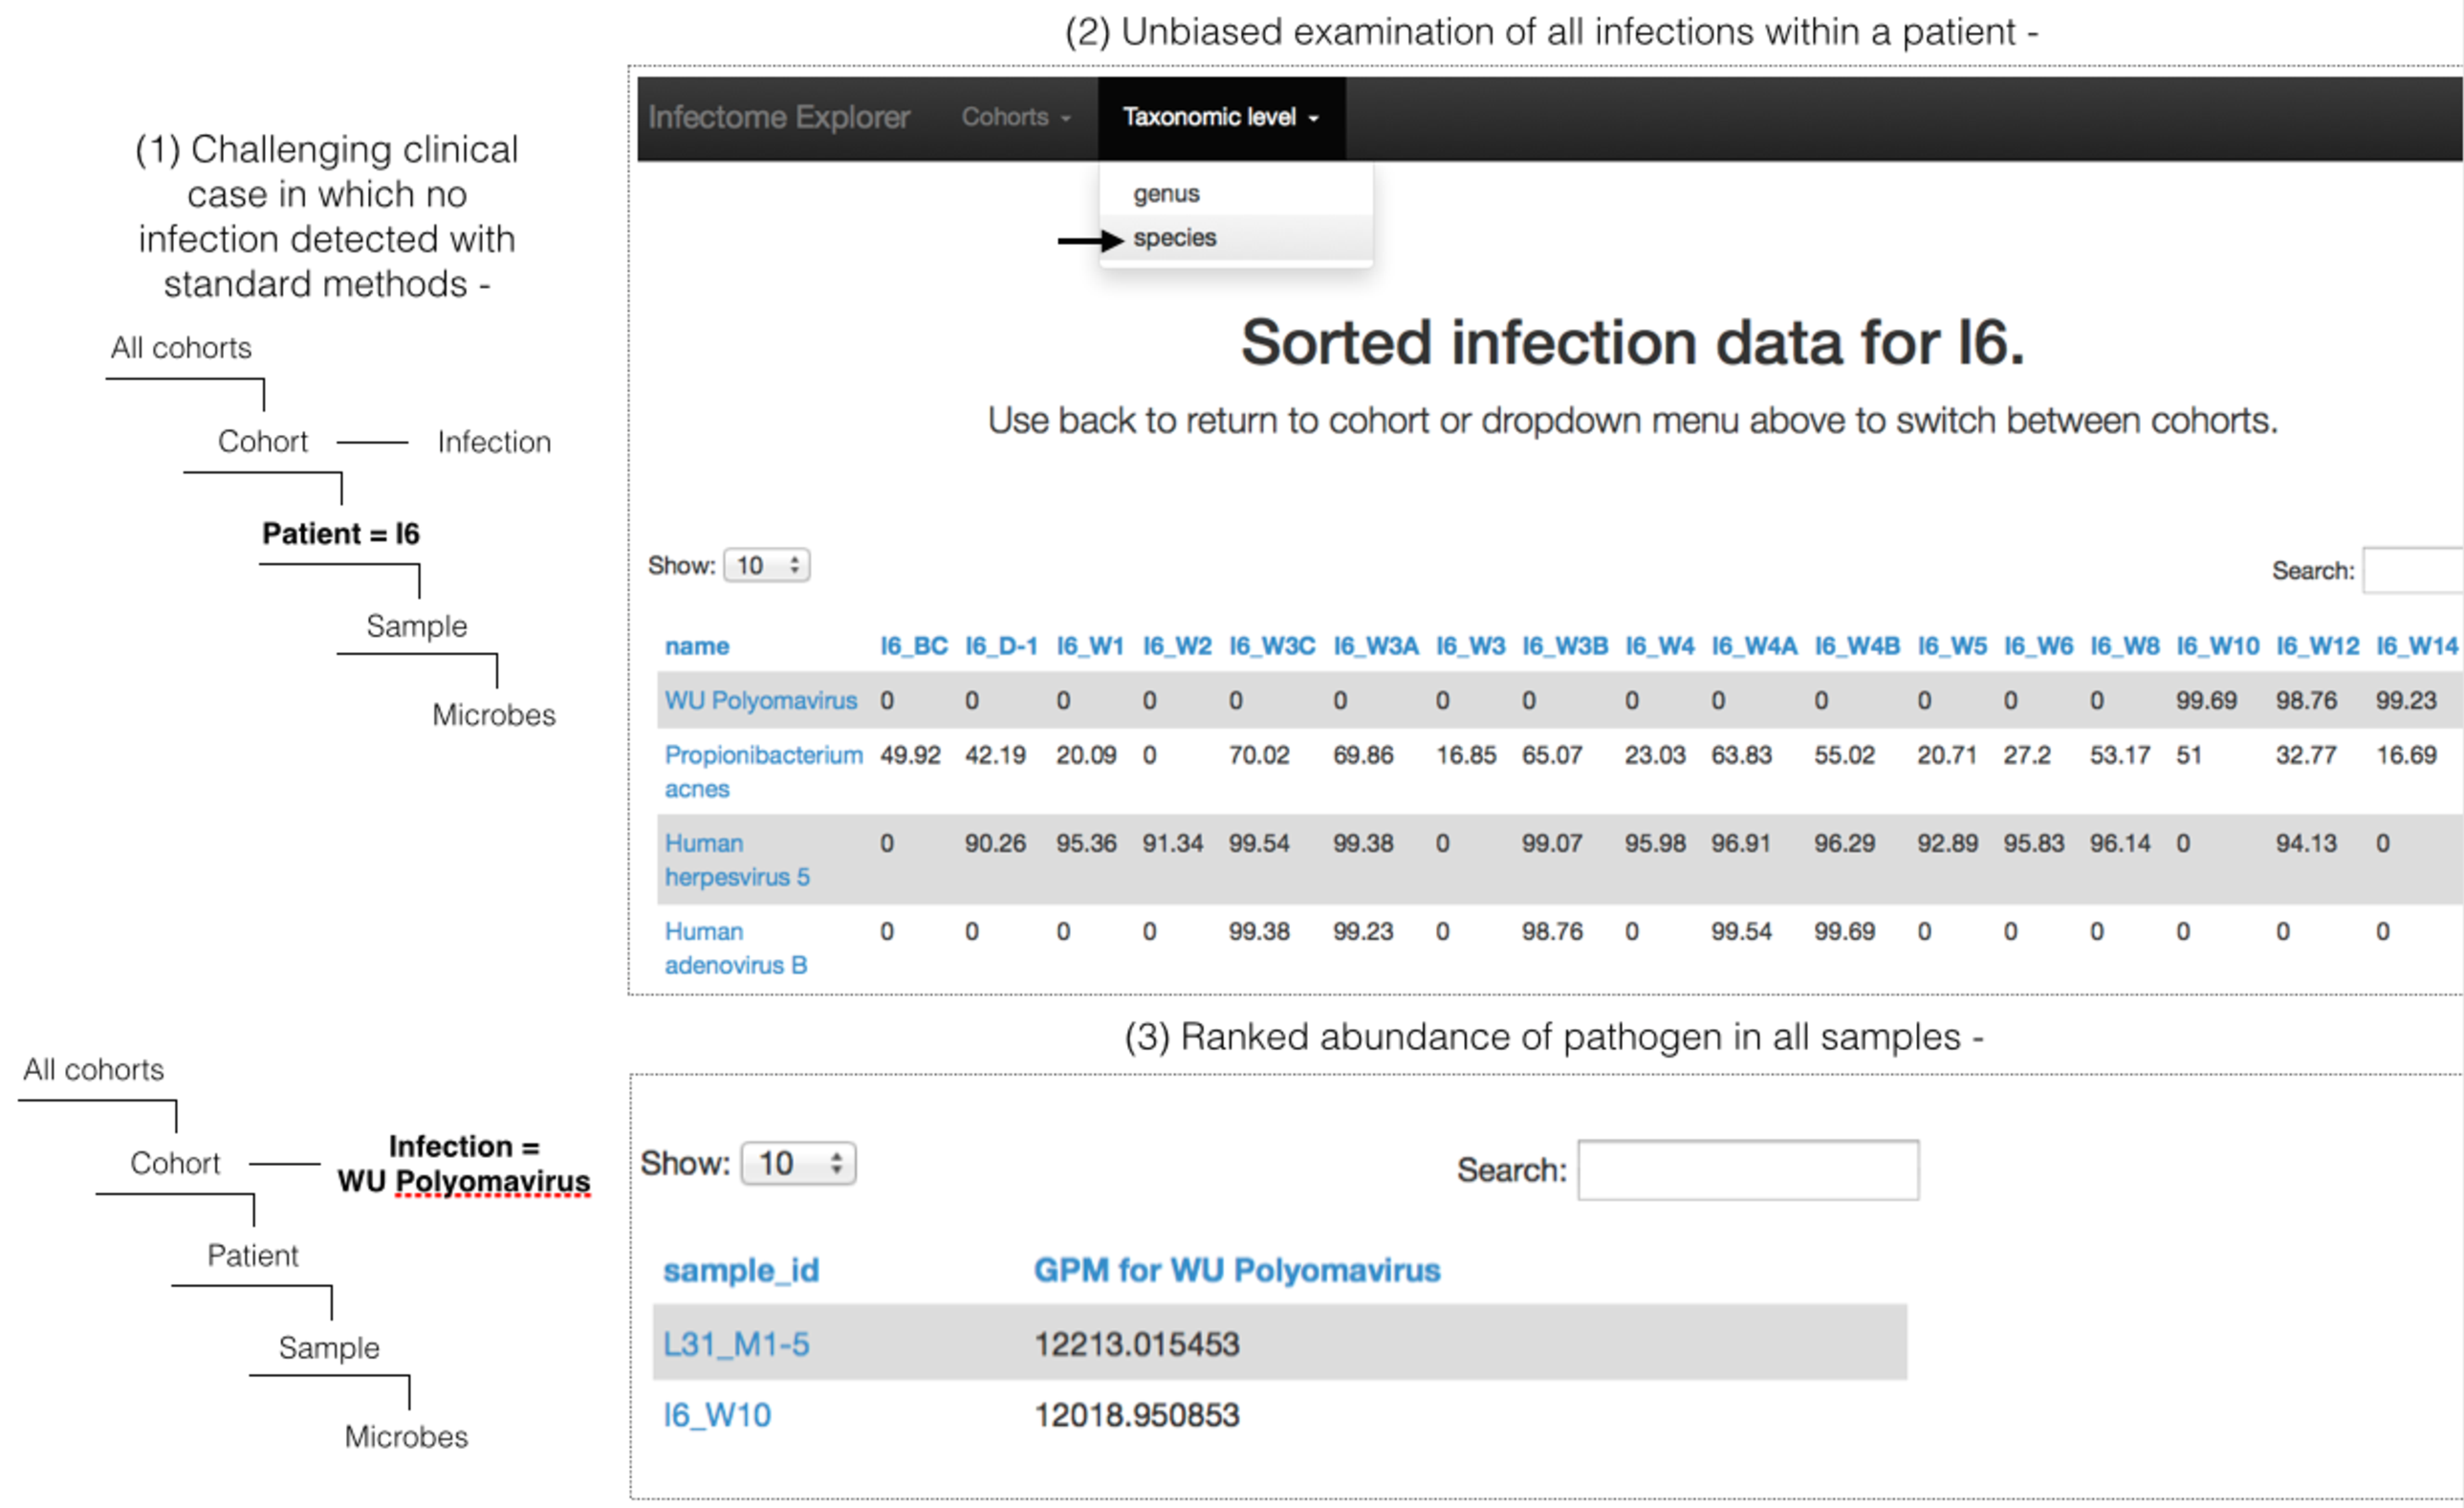
\includegraphics[width=150mm,scale=0.5]{Figures/Fig8}
\caption{Clinical use of infectome application}
\label{fig:Fig8}
\end{figure*}

To demonstrate clinical use for this application, we highlight the case of I6, a pediatric bone marrow patient with severe graft complications. We collected and processed longitudinal cell-free DNA samples over the course of post-transplant therapy. Using the patient-specific view, it was clear that I6 had a very high Polyomavirus load. Viewing the data at species-level, we can see WU Polyomavirus, a species that has been implicated in severe respiratory illnesses \cite{Kleines:2009gj} (Figure ~\ref{fig:Fig8}). 

Though the patient was tested for a different Polyomavirus (BK virus), those tests were negative. This situation is similar to a scenario recently described in the literature: NGS applied to cerebrospinal fluid within a deeply ill immunocomprised patient identified an exotic pathogenic bacteria, Leptospira, responsible for encephalitis and informed successful treatment \cite{Wilson:2014dv}. Unlike that case, I6 died prior to clinical intervention based upon this information. While it is not clear that WU Polyomavirus was responsible for the death of I6, it is clear that unbiased screening of potential pathogens in severe cases such as this one can reveal agents that escape clinical testing and serve as a powerful supplement to existing clinical assays.


